%\graphicspath{img}

\chapter{Présentation du problème et motivation} 

On présente d'abord le modèle, son comportement et les problématiques numériques associées, en détaillant l'ordre et le coût de certains schémas. 
On introduit ensuite le développement double-échelle qui va être la base de la prochaine partie, en précisant certains des problèmes qu'il pose et en évoquant certaines de ses propriétés. 

\section{Modèle, propriétés et soucis numériques}

On considère le modèle suivant 
\begin{equation} \label{pb:EDO_var_cent} \left\{
\begin{array}{rll}
\dot x\eeps =&\!\! f(x\eeps,z\eeps) , &x\eeps(0) = x_0\in\R^n \\ \displaystyle
\dot z\eeps =&\!\! \displaystyle -\inveps z\eeps + g(x\eeps,z\eeps), &z\eeps(0) = z_0\in\R^m
\end{array} \right.
\end{equation}
avec $f:\R^n\times\R^m \rightarrow \R^n,g:\R^n\times\R^m\rightarrow\R^m$ analytiques et $\epsilon$ un petit paramètre. 

Ce système est une simplification d'un autre, équivalent, qui fait apparaître $\inveps \Lambda z\eeps$ ($\Lambda$ diagonale positive) au lieu de $\inveps z\eeps$. 
Le système \eqref{pb:EDO_var_cent} peut ainsi être dérivé d'un laplacien, e.g. d'un problème de réaction-diffusion. 

On présente d'abord certaines propriétés de ce système, puis quelques méthodes numériques usuelles, en précisant leurs avantages et leurs défauts, et enfin on décrit le principe d'une méthode asymptotique moderne de \cite{castella2016formal} pour saisir encore un peu mieux le comportement du modèle. 


\subsection{Problème à variété centrale} 

Le comportement de la solution est résumé dans le \textit{théorème de variété centrale} et le \textit{principe de réduction}\cite{carr1982} suivant 

\begin{theorem} \label{thm:var_cent} 
Soit $B_R$ la boule de rayon $R$ et de centre $0$ dans $\R^n\times\R^m$. 
On suppose $f(0,0) = 0$ et $g(0,0) = 0$. 
Alors pour tout $R>0$, il existe $\epsilon^* > 0$ et $T>0$ tels que la solution $(x\eeps(t),z\eeps(t))$ de \eqref{pb:EDO_var_cent} existe pour tout $\epsilon\in]0,\epsilon^*]$, tout $t\in[0,T]$ et toute condition initiale $(x_0,z_0)\in B_R$. 

En outre, pour tout $\epsilon\in]0,\epsilon^*]$, il existe 
une fonctions $h\eeps:\R^n\rightarrow\R^m$ analytique de sorte que la variété 
$$ \mathcal{M} = \{(x,\epsilon h\eeps(x)), x\in\R^n\} $$
est invariante pour \eqref{pb:EDO_var_cent} dans le sens $(x_0,z_0)\in\mathcal{M}\cap B_R \Rightarrow \forall t\in[0,T], (x(t),z(t)) \in \mathcal{M}$. 
En particulier, $0_{\R^n\times\R^m}\in\mathcal{M}$ donc on l'appelle <<~variété centrale~>>. 
Par souci de simplicité, on confond l'ensemble $\mathcal{M}$ et la fonction $\epsilon h\eeps$ par cette appellation. 

Si on note $\varphi_t$ le flot en $t$ de l'EDO réduite 
\begin{equation} \label{eq:EDO_reduite}
\dot{\nu} = f(\nu,\epsilon h\eeps(\nu))
\end{equation}
alors il existe $\mu > 0$ tel que pour tous $(x_0,z_0)\in B_R, \epsilon\in]0,\epsilon^*]$, 
il existe une condition initiale dite réduite $x_0\eeps \in\R^n$ telle que 
$$ \forall t\in[0,T], \quad x(t) = \varphi_t(x_0\eeps) + \O\left(e^{-\mu t/\epsilon}\right) \quad\text{et}\quad z(t) = \epsilon h(\varphi_t(x_0\eeps)) + \O\left( e^{-\mu t/\epsilon}\right). $$
\end{theorem}

En d'autres termes, le système converge très rapidement (à vitesse $e^{-t/\epsilon}$) vers un état <<~réduit~>> où $z\eeps$ est entièrement déterminé par $x\eeps$ \textit{via} la relation $z\eeps = \epsilon h\eeps \circ x\eeps$. 
On ne démontrera pas ce théorème bien connu mais on l'illustre par des exemples en annexe~\ref{sec:ann_exemples}. 

Présentons un exemple précis et vérifions la convergence vers la variété. On choisit $n,m = 1$, 
\begin{equation} \label{pb:edo_partic_1}
\left\{ \begin{array}{l}
f(x,z) = -x^3(z-z^3/3) \vphantom{\displaystyle\sum_0} , \\
g(x,z) = x(1-z^2/2) 
\end{array} \right. 
\qquad \text{et} \qquad 
\left\{ \begin{array}{l}
x_0 = 0,8 \vphantom{\displaystyle\sum_0} \\
z_0 = 0,05 
\end{array} \right.
\end{equation}
cet exemple étant traité chez \cite{castella2016formal}. 
On trace la solution sur $[0,1]$ pour quelques valeurs de $\epsilon$ ainsi que la variété associée afin de vérifier ce comportement. 
Comme on ne connaît pas de solution analytique, on utilise une implémentation \bsc{Matlab} du schéma Radau IIa\cite{codeRADAU} avec une tolérance absolue de $10^{-16}$ et une tolérance relative de $10^{-13}$ pour calculer une solution quasi-exacte. 
\begin{figure}[!h]
\centering\label{fig:sol_periode_transitoire}
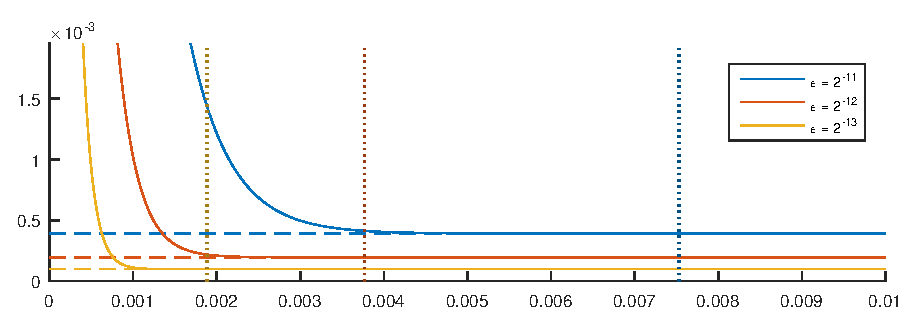
\includegraphics[width=.85\textwidth]{img/chap1/solution_transition_v2.eps}
\caption{Solution $z$ en fonction du temps et la solution sur la variété associée $z_{\infty}:t\mapsto \epsilon h\eeps \circ \varphi_t(x_0\eeps)$, pour $\epsilon = 2^{-11},2^{-12},2^{-13}$. La fin du régime transitoire est indiquée en pointillés comme l'instant $t_0$ à partir duquel $\forall t\geq t_0,\ |z(t)-z_{\infty}(t)| \leq 10^{-8}$.}
\end{figure}

On observe bien dans cet exemple une convergence exponentielle de $z$ vers le régime permanent qu'est la variété centrale $z_{\infty} = \epsilon h\eeps(x)$, avec un régime transitoire de durée d'ordre $\epsilon$. 
En effet on voit que diviser $\epsilon$ par 2 divise également la durée du régime transitoire par 2. 
Il y a bien deux dynamiques en jeu: celle du régime transitoire, en $e^{-t/\epsilon}$ et celle du régime permanent, qui dépend de $\epsilon$ de façon \textit{non raide}. \\


\subsection{Méthodes numériques usuelles} \label{subsec:meth_num_usuelles}

On considère ici principalement les méthodes numériques à pas de temps uniforme. 
On suppose dans nos exemples que le système \eqref{pb:EDO_var_cent} admet une solution bornée sur $[0,T]$, et on définit le pas de temps $\dt = T/N$ avec $N$ le nombre de sous-divisions de l'intervalle. On note $t_n = n\dt,\ n=0,\ldots,N$. 
Pour un schéma donné, on s'intéressera aux erreurs locales $\lex_{n+1}, \lez_{n+1}$ définies par 
$$ \lex = |x_1 - x(\dt)|, \quad \lez = |z_1 - z(\dt)| $$
où $|\cdot|$ est la norme euclidienne de $\R^n$ ou de $\R^m$ et $x_1,z_1$ sont obtenus par le schéma à partir de $x_0,z_0$. 

Les méthodes numériques usuelles à pas fixe permettent d'obtenir des erreurs en $\Delta t^p/\epsilon^q$, $p,q > 0$. 
Lors de la première partie de mon stage, j'ai implémenté et expérimenté avec quelques uns de ces schémas. 
J'ai aussi évalué les performances d'un schéma implicite-explicite \textit{ad hoc}, d'un splitting de Strang et d'un schéma à pas de temps adaptatif. 

On présente certains de ces schémas de façon plus poussée en annexe \ref{chap:erreus_schemas}, avec des études théoriques et numériques d'erreurs. 
En particulier, des graphes d'erreurs sont disponibles. 

\subsubsection{Schémas explicites à pas fixe}

L'erreur locale $\ell e^{(x)}, \ell e^{(z)}$ d'un schéma d'Euler explicite avec $\epsilon < 1$ fixé est 
$$ \lex = \O(\dt^2/\epsilon), \qquad \lez = \O(\dt^2/\epsilon^2). $$ 
Il est intéressant de noter que cela ne génère pas nécessairement une erreur finale en $\epsilon^{-2}$ sur $z$, puisque $z$ cesse rapidement d'être raide. 

\subsubsection{Implicite-explicite \textit{ad hoc}}

Une idée qui peut sembler naturelle est d'impliciter la partie raide pour garder explicite la partie non-linéaire (dans $f,g$). 
Nos calculs et simulations (en annexe \ref{sec:ann_schemas_sep_vitesses}) donnent les erreurs locales 
$$ \lex = \left\{ \begin{array}{ll} 
\O(\dt) &\quad \text{si } \epsilon\ll\dt \\ 
\O(\dt^2/\epsilon) &\quad \text{si } \dt\ll\epsilon 
\end{array} \right. ,
\qquad \lez = \left\{ \begin{array}{ll} 
\O(\epsilon/\dt) &\quad \text{si } \epsilon\ll\dt \\
\O(\dt^2/\epsilon^2) &\quad \text{si } \dt\ll\epsilon
\end{array} \right. $$
On voit qu'il faut toujours imposer $\dt\ll\epsilon$ pour avoir une erreur raisonnable. 
L'avantage est que le schéma est bien plus stable que le schéma complètement explicite, et il est aussi plus rapide qu'un schéma d'Euler implicite usuel. 

\subsubsection{Splitting de Strang}

La partie raide du système est essentiellement contenue dans le terme $-\inveps z$, et donc on propose de séparer le système en deux parties pour le splitting 
$$ \left\{\begin{array}{rl}
\dot x = & 0 \\ \dot z =& -\inveps z
\end{array}\right. \qquad\qquad 
\left\{\begin{array}{rl}
\dot x = & f(x,z) \\ \dot z =& g(x,z)
\end{array}\right. $$
On voit qu'on peut résoudre la première partie exactement à moindre coût, et la deuxième avec un schéma Radau IIA avec une tolérance faible. 
On peut alors supposer que l'erreur provient uniquement du splitting, et donc on calcule une erreur locale théorique d'ordre $\O(\dt^3/\epsilon^2)$ sur $(x,z)$ dans le cas $f,g$ linéaires. 
Cette vitesse de convergence est bien vérifiée pour $x$ sur nos exemples, mais l'ordre est dégénéré pour $z$ (sûrement à cause des non-linéarités). 
Ainsi on obtient 
$$ \lex = \O(\dt^3/\epsilon^2) \qquad \text{et} \qquad 
\lez = \O(\dt^2/\epsilon) $$
Les erreurs globales $e^{(x)},e^{(z)}$ respectent 
$$ e^{(x)} = \O(\dt^2/\epsilon) \qquad \text{et} \qquad e^{(z)} = \O(\dt^2/\epsilon^2) $$
ce qui est bien une convergence d'ordre 2. 


\subsubsection{Pas de temps adaptatif}

Une dernière méthode usuelle que nous avons considérée est une méthode de Runge-Kutta imbriqués d'ordre 3, à partir de RK4 avec la règle des 3/8. Son tableau de Butcher est donné par 
\begin{center}
\begin{tabular}{c|ccccc}
 0  &  0   &  0  &  0  &  0  &  0  \\
1/3 & 1/3  &  0  &  0  &  0  &  0  \\
2/3 & -1/3 &  1  &  0  &  0  &  0  \\
 1  &  1   & -1  &  1  &  0  &  0  \\
 1  & 1/8  & 3/8 & 3/8 & 1/8 &  0  \\ \hline
    & 1/8  & 3/8 & 3/8 & 1/8 &  0  \\ 
    & 1/12 & 1/2 & 1/4 &  0  & 1/6
\end{tabular}
\end{center}
qui nous donne deux estimations $\hat{x}_{n+1},\hat{z}_{n+1}$ et $\tilde{x}_{n+1},\tilde{z}_{n+1}$ (notons que la colonne des coefficients en temps à gauche n'est pas utile dans notre cas). On calcule la différence entre ces deux estimations pour obtenir un pas de temps adapté  
$$ \dt_{\text{opt}} = 0.9 \dt \left(\dfrac{Tol}{|\hat{u}_{n+1}-\tilde{u}_{n+1}|}\right)^{1/4} $$
où $u = \begin{pmatrix} x \\ z \end{pmatrix}$. \\

Ce choix de pas de temps est classique et est présenté à maintes reprises dans \cite{hairer1991}. 
Le cas échéant, il est expliqué en annexe \ref{subsec:ann_rke}. 
Après implémentation, on observe un coût en $\O(1/\epsilon)$ indépendant du facteur de tolérance pour $\epsilon$ petit (fig. \ref{fig:cout_rke} en sec. \ref{subsec:ann_rke}), ce qui rend finalement ce schéma aussi (mal) adapté que les autres. 


\subsubsection{Schéma Radau IIA}
On utilise ce schéma implicite à pas de temps adaptatif pour calculer nos solutions de référence. 
Pour l'implémentation, on utilise un code \bsc{Matlab} \cite{codeRADAU} qui est une traduction du code \bsc{Fortran} de E. Hairer et G. Wanner appliquant la méthode Radau IIA \cite[\textit{sec}.~IV.5]{hairer1991}.

On se sert de ce code pour calculer nos solutions de références et on n'évalue pas sa convergence, mais on peut mesurer son coût en fonction de $\epsilon$. 
\begin{figure}[!h]
\centering
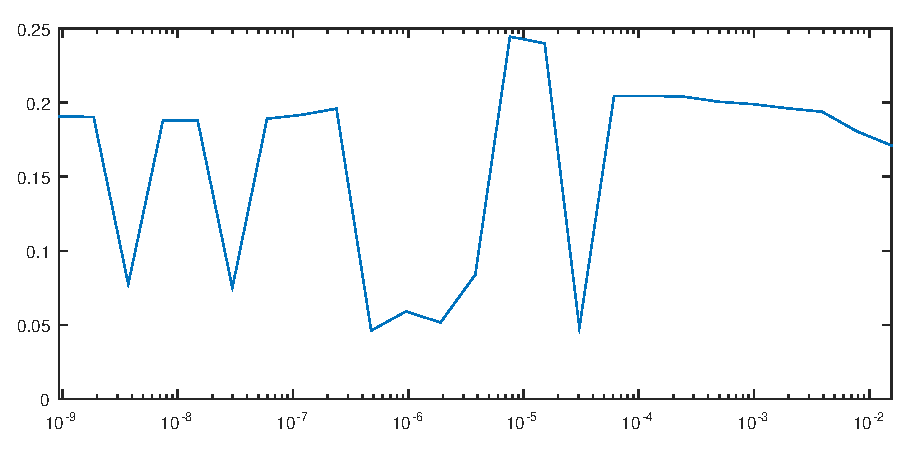
\includegraphics[width=.8\textwidth]{img/chap1/cost_radau.eps}
\caption{Temps du calcul d'une solution $u\eeps$ de référence avec le schéma Radau IIA pour différentes valeurs de $\epsilon$.}
\end{figure}
Il est évident que la valeur de $\epsilon$ a une influence sur le temps de calcul, mais il est impossible de déceler une relation nette. 

On pourrait se dire que ce schéma est suffisant, mais nous allons poursuivre notre étude dans une autre direction pour 
\begin{enumerate}
\item essayer de trouver des méthodes au coût indépendant de $\epsilon$ et
\item trouver des méthodes \textit{uniformément précises} qui pourront nous aider à attaquer d'autres problèmes raides plus complexes par la suite. 
\end{enumerate}


\subsection{Méthodes asymptotiques}

Des méthodes plus modernes et plus formelles cherchent à déterminer l'expression quasi-exacte de la variété $\epsilon h\eeps$ ainsi que la condition initiale modifiée $x_0\eeps$. 

Il est intéressant de noter que $h\eeps$ respecte la relation 
\begin{equation} \label{eq:formule_variete}
\forall x\in\R^n, \qquad \epsilon(h\eeps)'(x)\cdot f(x,\epsilon h\eeps(x)) = - h\eeps(x) + g(x,\epsilon h\eeps(x)) 
\end{equation}
et ainsi, à l'aide de développements limités successifs sur la seconde variable de $f$ et de $g$, on obtient une formulation en puissances de $\epsilon$ pour $h\eeps$. 
En particulier, on a 
$$ h\eeps(x) = g(x,0) + \epsilon \big(\dpz g(x,0)\cdot g(x,0) - \dpx g(x,0)\cdot f(x,0) \big) + \O(\epsilon^2). $$

Il est bien plus difficile de déterminer $x_0\eeps$, puisque cela demande de connaitre l'état du système après la période transitoire pour ensuite <<~remonter~>> le flot de l'équation différentielle réduite \eqref{eq:EDO_reduite}. 
Une méthode a été trouvée récemment dans \cite{castella2016formal} et permet d'obtenir un développement de cette condition modifiée jusqu'à un certain ordre $\epsilon^k$. 
Cette approche est très utile lorsqu'on ne cherche pas à capturer la période transitoire du système et que $\epsilon$ est petit. Elle permet de réduire la complexité du problème \textit{a priori} par principe de réduction (i.e. en se limitant à la variété, où $z$ est déterminé par $x$), et fournit un système dont la seule raideur provient de $f$. Cependant, elle est difficile à implémenter du fait de sa nature algébrique complexe, et n'est pas adaptée si l'on veut capturer la phase transitoire dans une simulation. 

On obtient néanmoins une erreur en $\O(\dt^p + \epsilon^q)$ sur $(x,z)$ après la phase transitoire. \\

Dans \cite{castella2016formal}, la méthode permet également de trouver un nouveau modèle asymptotiquement stable où $x$ est indépendante, peu raide et où on peut calculer $z$ avec le nouveau modèle. 
L'équation sur $z$ peut être raide, en revanche, et les calculs restent assez formels et complexes.
On utilise les résultats de cet article en annexe \ref{subsec:ann_asymp} pour vérifier que l'erreur est la bonne et pour illustrer cette approche. 



\section{Introduction au développement double-échelle}


De la même manière que pour le cas périodique dans \cite{chartier2015UA}, on considère $u = (x,z)$ comme évaluation particulière d'une fonction $U = (X,Z)$ à deux variables $t,\tau$, 
$$ u(t) = U(t,t/\epsilon) $$
pour laquelle on doit trouver un bon ensemble de définition. 
Cette décomposition est aussi à la base de la méthode d'homogénéisation. 
Dans le cas périodique de période $P$, il était naturel de faire évoluer la seconde variable $\tau$ dans $\R/P\mathbb{Z}$, puisqu'elle représentait la partie périodique du problème. 
On verra quel ensemble choisir ici. 

Quel que soit cet ensemble, on trouve que $X,Z$ sont solutions d'un problème de transport 
\begin{equation} \label{eq:trsp_XZ}
\begin{array}{c} \displaystyle
\dpt X + \inveps \dptau X = f(X,Z) 
\\ \displaystyle
\dpt Z + \inveps \dptau Z = -\inveps Z + g(X,Z)
\end{array}
\end{equation}
où la seule donnée qu'on connaît est $X(0,0) = x_0$ et $Z(0,0) = z_0$. \\

On va d'abord discuter des conditions supplémentaires dont on a besoin pour que le problème soit bien posé avec $\tau$ dans un intervalle ou ensemble qu'on choisira, puis on exhibera des conditions pour que le problème soit bien posé et que sa solution soit d'une certaine régularité qu'on précisera. 


\subsection{Nouvelles problématiques}

Comme nous l'avons déjà remarqué, la première difficulté qui se pose est de choisir l'ensemble de définition pour $\tau$. 
Ce choix est en réalité assez simple. 
Dans le cas périodique, l'ensemble de définition de $\tau$ était indépendant de $\epsilon$. 
On souhaite garder cette propriété dans le cas non-périodique, et on observe que si $x,z$ sont définies sur $[0,T]$, $\tau$ parcourt $[0,T/\epsilon]$. 
Ainsi on choisit $\R_+$ comme ensemble pour $\tau$, i.e. on aimerait que $U$ soit définie sur $[0,T]\times\R_+$, i.e. 
$$ U : [0,T]\times\R_+ \rightarrow E := \R^n\times\R^m . $$

On peut maintenant analyser le problème \eqref{eq:trsp_XZ} dans $[0,T]\times\R_+$. 
Il s'agit d'un problème de transport à vitesse constante $1/\epsilon$, donc l'analyse se fera surtout par méthode des caractéristiques. 
Considérons dans un premier temps un problème indépendant de $\epsilon$, 
$$ \dpt u + \dptau u = F(t,\tau,u) $$
avec $F:[0,T]\times\R_+\times E \rightarrow E$. 
On voit qu'on peut obtenir un problème similaire à partir de \eqref{eq:trsp_XZ} avec le changement de variable $\tau \leftarrow \epsilon\tau$, et en fixant $\epsilon$ pour obtenir $F$ indépendante de $\epsilon$. 
Ce problème est donc, à $\epsilon$ fixé, plus général que celui sur $X,Z$. \\


L'aspect de $[0,T]\times\R_+$ fait qu'on doit s'intéresser tout particulièrement à la droite $(t,t),t\in[0,T]$. 
Les droites caractéristiques sont de la forme $(t,\tau+t),\tau\in\R_+,t\in[0,T]$ sous cette diagonale et $(t+t_0, t),t_0\in[0,T],t\in[0,T-t_0]$ au dessus. 
On voit ainsi que certaines caractéristiques ont leur origine sur la demi-droite $(0,\tau),\tau\geq 0$ et d'autre sur le segment $(t_0,0),t_0\in[0,T]$, 
donc pour pouvoir résoudre le problème il faut nécessairement une condition initiale \textit{et} une condition au bord. 

C'est une différence majeure avec le problème périodique, qui ne nécessitait pas de condition au bord. 
Sans condition au bord, la régularité de la condition initiale est transmise naturellement à la solution. Nous allons voir très rapidement que ce n'est pas le cas ici. 
Considérons le problème avec une régularité presque minimale \\
\textit{Trouver $(\overline{T},u)\in]0,T]\times C^0([0,\overline{T}]\times\R_+)$ tel que pour tout $(t,\tau)\in[0,\overline{T}]\times\R_+$ on ait }
\begin{equation} \label{pb:trsp_u_no_eps}
\dpt u + \dptau u = F(t,\tau,u) 
\end{equation}
avec les conditions initiales $u(0,\tau) = u_I(\tau), \tau\in\R_+$ et les conditions au bord $u(t,0) = u_B(t), t\in]0,\overline{T}]$. 
La restriction à $\overline{T} \leq T$ permet d'assurer qu'on ne cherche pas nécessairement une solution sur $[0,T]\times\R_+$ entier, où l'existence ne serait pas toujours garantie à cause des non-linéarités de $F$. 

Admettons qu'on choisisse $u_I$ et $u_B$ quelconques dans $C^0(\R_+)$ et $C^0([0,T])$ respectivement. 
Il est évident que si $u_I(\tau = 0) \neq u_B(t=0)$, la solution (si elle existe) ne peut pas être continue, puisqu'alors $\lim_{\delta\rightarrow 0^+} u(\delta,0) \neq u(0,0)$. 
Réciproquement, 
\begin{lemma} \label{thm:pb_gen_bien_pose}
Si $u_B\in C^0_b([0,T])$, $u_I \in C^0_b(\R_+)$ avec $u_B(t=0) = u_I(\tau = 0) =: u_0$, si $F$ est localement lipschitzienne par rapport à $u$, continue de $[0,T]\times\R_+\times E$ dans $E$, bornée par rapport à $\tau$, alors le problème \eqref{pb:trsp_u_no_eps} est bien posé au sens suivant: 
 
Pour tout facteur $\kappa > 1$, il existe un temps $\Tk\in]0,T]$ tel que le problème (\ref{pb:trsp_u_no_eps}) a une unique solution $u$ dans $C^0([0,\Tk]\times\R^+)$, qui respecte l'inégalité 
\begin{equation}
\forall t\in [0,T_{\kappa}], \qquad \|u(t,\cdot) \|_{\Linftau} \leq \kappa\, \max\left\{ \|u_I\|_{\Linftau}, \|u_B\|_{\Linft} \right\}. 
\end{equation}

Si en outre $F$ respecte $\forall (t,\tau,u)\in [0,T]\times\R_+\times E, |F(t,\tau,u)| \leq C_F |u| + D_F$ pour des constantes $C_F,D_F \geq 0$, alors il existe une unique solution $u$ dans $C^0([0,T]\times\R_+)$ qui vérifie 
\begin{equation}
\forall t\in[0,T], \|u(t,\cdot)\|_{\Linftau} \leq \left( \max\left\{ \|u_I\|_{\Linftau}, \|u_B\|_{\Linft} \right\} + t D_F \right) e^{t C_F}. 
\label{eq:ineg_lin_u}
\end{equation}

\end{lemma}

\begin{proof}
La preuve utilise les droites caractéristiques du problème et ne pose pas de difficultés particulières. 
Néanmoins, sa bonne compréhension nécessite de séparer les fonctions caractéristiques qui ont comme origine une condition initiale de celle qui prennent une condition au bord. 
Cette distinction rend la preuve un peu longue et elle se trouve donc en annexe \ref{chap:ann_preuve}, p. \pageref{chap:ann_preuve}. 
\end{proof}

Exhibons maintenant des conditions supplémentaires sur $u_B$ et $u_I$ pour que la solution $u$ du problème soit de classe au moins $C^2$. 

\subsection{Caractère bien posé dans $C^2$} \label{subsec:carac_C2_gen}

Pour simplifier l'étude, on suppose maintenant $F$ indépendante de $t,\tau$, i.e. $F:E\rightarrow E$. 
Avec $\kappa$ fixé, quitte à ce que ce soit au sens des distributions dans $L^{\infty}([0,\Tk]\times\R_+)$, on peut dériver le problème de transport \eqref{pb:trsp_u_no_eps} selon $t$ pour obtenir que $\dpt u\eeps =: v\eeps$ vérifie 
\begin{equation} 
\begin{array}{c}
\displaystyle
\dpt v + \dptau v = \dpu F(u)\cdot v \vphantom{\int_0^1}
\\ \displaystyle
v(0,\tau) = F(u_I(\tau)) - u_I'(\tau) \quad \text{et} \quad v(t,0) = u_B'(t)
\end{array}
\label{pb:trsp_v_no_eps}
\end{equation}
D'après l'étude précédente, il apparaît immédiatement que pour que $v$ soit continue, il faut non seulement avoir $u_I\in C^1(\R_+)$, $u_B\in C^1([0,\Tk])$  
et $\dpu F$ continue de $E$ dans $L(E,E)$, mais aussi 
\begin{equation}
u_B'(t=0) + u_I'(\tau = 0) = F(u_0)
\label{eq:compat_ord1}
\end{equation}
où $u_0 := u_I(\tau = 0) = u_B(t = 0)$. 
Admettons que nos conditions initiale et au bord sont bien choisies de sorte que $v$ ainsi définie soit continue (i.e. de sorte que la relation \eqref{eq:compat_ord1} soit vérifiée). 
Alors on peut dériver à nouveau pour obtenir une équation sur $\dpt v =: w$ 
\begin{equation} \label{pb:trsp_w_no_eps}
\begin{array}{lc}
&\displaystyle
\dpt w + \dptau w = %\dpt^2 F(t,\tau,u) + \dpt\dpu F(t,\tau,u) +
\dpu^2 F(u)\cdot (v,v) + \dpu F(u)\cdot w \vphantom{\int_0^1}
\\ & \displaystyle
w(0,\tau) = %\dpt F_0(\tau,u_I) + 
\dpu F(u_I)\cdot (v(0,\tau) - u_I') %- \dptau F_0(\tau,u_I) 
+ u_I'' \vphantom{\int_0^1} 
\quad %\\
\text{et} \quad w(t,0) = u_B''(t)
\end{array}
\end{equation}
où %$F_0(\cdot,\cdot) = F(0,\cdot,\cdot)$ et 
$u_I,u_I'$ et $u_I''$ sont évaluées en $\tau$ dans la condition initiale. On voit que la condition de continuité peut alors s'écrire 
\begin{equation} \label{eq:compat_ord2} 
%\dpt F(0,0,u_0) + 
\dpu F(u_0)\cdot u_B'(0) - u_B''(0) = %\dptau F(0,0,u_0) + 
\dpu F(u_0)\cdot u_I'(0) - u_I''(0). 
\end{equation}
On peut alors exhiber des conditions suffisantes pour que la solution soit de classe $C^2$ dans le problème \eqref{pb:trsp_u_no_eps}, avec $F$ indépendante de $t,\tau$. \\


\begin{theorem} \label{thm:regularite_u_no_eps}
Si $u_B\in C^2_b([0,T])$, $u_I\in C^2_b(\R_+)$, 
si $F$ (resp. $\dpu F$ et $\dpu^2 F$) est continue de $E$ dans $E$ (resp. $L(E,E)$ et $L(E^2,E)$), et enfin si 
$$u_B(0) = u_I(0) =: u_0, \qquad u_B'(0) + u_I'(0) = F(u_0),$$
$$ \text{et}\quad %\dpt F(0,0,u_0) + 
\dpu F(u_0)\cdot u_B'(0) - u_B''(0) = %\dptau F(0,0,u_0) + 
\dpu F(u_0)\cdot u_I'(0) - u_I''(0) $$
alors le problème \eqref{pb:trsp_u_no_eps} est bien posé et régulier au sens suivant :

Pour tout facteur $\kappa > 1$, il existe un temps $\Tk\in]0,T]$ tel que le problème (\ref{pb:trsp_u_no_eps}) a une unique solution $u$ dans $C^2([0,\Tk]\times\R^+)$, qui respecte l'inégalité 
\begin{equation}
\forall t\in [0,T_{\kappa}], \qquad \|u(t,\cdot) \|_{\Linftau} \leq \kappa\, \max\left\{ \|u_B\|_{\Linft}, \|u_I\|_{\Linftau} \right\}. 
\label{eq:ineg_u_no_eps}
\end{equation}
et avec $C_0' = \sup\left\{\vertiii{\dpu F(u(t,\tau))},\, (t,\tau)\in [0,\Tk]\times\R_+ \right\}$ on a 
\begin{equation}
\forall t\in[0,\Tk], \qquad \|\dpt u(t,\cdot)\|_{\Linftau} \leq \max \left\{\|u_B'\|_{\Linft}, \|v_I\|_{\Linftau} \right\} e^{t C_0'},
\end{equation}
où $v_I = F(u_I) - u_I'$. De la même manière, avec $C_1'' = \| \dpu^2 F(u)\cdot(v,v )\|_{L_{t,\tau}^{\infty}}$, on a 
\begin{equation}
\forall t\in[0,\Tk], \qquad \|\dpt^2 u(t,\cdot)\|_{\Linftau} \leq \left( \max \left\{\|u_B''\|_{\Linft}, \|w_I\|_{\Linftau} \right\} + t C_1'' \right) e^{t C_0'}
\end{equation} 
où $w_I = \dpu F(u_I)\cdot(v_I - u_I') + u_I''$. 
\end{theorem}

\begin{proof}
Soit $\kappa > 1$. Le lemme \ref{thm:pb_gen_bien_pose} assure l'existence de $(\Tk,u)\in ]0,T]\times C^0_b([0,\Tk]\times\R_+)$ vérifiant l'inégalité souhaitée. 
On peut ensuite appliquer le cas affine du lemme \ref{thm:pb_gen_bien_pose} successivement aux problèmes \eqref{pb:trsp_v_no_eps} puis \eqref{pb:trsp_w_no_eps} en considérant $u$ puis $v$ comme des paramètres, et on obtient $\dpt u \in C^0_b([0,\Tk]\times\R_+)$ puis $\dpt^2 u\in C^0_b([0,\Tk]\times\R_+)$), avec les bornes souhaitées. 

On remarque enfin 
$$\dptau u = F(u) - \dpt u, \quad\dptau \dpt u = \dpu F(u)\cdot \dpt u - \dpt^2 u \quad\text{et}\quad \dptau^2 = \dpu F(u)\cdot \dptau u - \dpt \dptau u$$
donc la régularité de $u,\dpt u$ et $\dpt^2 u$ se propage aux dérivées première et seconde de $u$ pour assurer $u\in C^2([0,\Tk]\times\R_+)$. 

\end{proof}

On voit ainsi que les conditions initiale et au bord sont intimement liées. 
Puisqu'on est libre de choisir les deux, on se dit que le plus simple est de fixer l'une des deux pour ensuite choisir l'autre de manière adaptée. 
On choisit de se concentrer d'abord sur la condition initiale, pour des raisons qui vont apparaître rapidement. 

\begin{remark}
Pour avoir une solution d'ordre $C^3$, on doit respecter 
$$
u_B''' + u_I''' = \dpu^2 F(u_0)\cdot(u_B',u_B') + \dpu^2 F(u_0)\cdot(u_I',u_I') - \dpu^2 F(u_0)\cdot(u_B',u_I') + \dpu F(u_0)\cdot(u_B''+u_I'') .
$$
\end{remark}

\subsection{Condition initiale ou condition au bord?}

Le but est de trouver de bonnes données (conditions initiale et au bord) de sorte à avoir $X,\dpt X, \dpt^2 X$ et $Z,\dpt Z, \dpt^2 Z$ uniformément bornés sur $[0,\Tk]\times\R_+$ afin de pouvoir trouver un schéma numérique uniformément précis (UP) d'ordre 1, i.e. d'erreur globale $\O(\dt)$ à constante indépendante de $\epsilon$. 
L'inspiration provient naturellement des méthodes d'Euler pour lesquelles l'erreur locale est d'ordre $\dt^2 (\|\dpt^2 X\| + \|\dpt^2 Z\|)$. 

Mettons d'abord le problème \eqref{eq:trsp_XZ} sous la forme 
\begin{equation} \label{eq:trsp_U_L}
\dpt U + \inveps LU = F(U) 
\end{equation} 
avec $U = \begin{pmatrix} X \\ Z \end{pmatrix}$ et $F(U) = \begin{pmatrix} f(X,Z) \\ g(X,Z) \end{pmatrix}$, des conditions initiale $U_I$ et au bord $U_B$, et $L$ un opérateur bien choisi. En l'occurrence, 
$$ LU := \begin{pmatrix} L_x X \\ L_z Z \end{pmatrix} := \begin{pmatrix} \dptau X \\ e^{-\tau} \dptau [e^{\tau} Z] \end{pmatrix}. $$
On admet pour le moment qu'on peut borner $\dpt U$ en fonction de $\inveps LU_I$ puisque $\dpt U(0,\tau) = F(U_I) - \inveps LU_I$ et que le lemme \ref{thm:regularite_u_no_eps} va dans ce sens. 
On voit alors qu'un mauvais choix de la condition initiale peut faire apparaître un facteur $1/\epsilon$ dans $\dpt U$. 

On voit en revanche que pour la valeur au bord de $\dpt U$, seule la dérivée $U_B'$ compte: il n'y a pas de facteur $1/\epsilon$ qui apparaît. Même pour les dérivées en $\tau$, on a $\dptau U(t,0) = -U_B + \epsilon(F(U_B) - U_B')$, donc $U_B$ semble ne pouvoir faire apparaître un facteur $1/\epsilon$ que si sa dérivée en fait apparaître un. 

En outre, si $U_I$ est telle que $\dpt U(0,\cdot) =: V_I(\cdot)$ et $\dpt^2 U(0,\cdot) =: W_I(\cdot)$ sont définies (il suffit d'avoir $U_I \in C^2$) et uniformément bornées, i.e. $$\exists C>0,\forall \epsilon\in]0,\epsilon^*], \|V_I\|_{\Linftau},\|W_I\|_{\Linftau} \leq C$$
alors on peut définir 
\begin{equation} \label{eq:CB_UVW}
U_B(t) = U_I(0) + t V_I(0) + \frac 1 2 t^2 W_I(0)
\end{equation}
pour obtenir une solution de classe $C^2$ qui, on l'espère (et on le montrera ensuite), est uniformément bornée sur $[0,T]\times\R_+$ avec ses dérivées $\dpt U, \dpt^2 U$ qui le sont aussi. 